\section{%
  单选题：本题共 8 小题，每小题 5 分，共 40 分。
  在每小题给出的四个选项中，只有一项是符合题目要求的。
}

% 1.
\begin{question}
  已知 $\vec{a}=(2,4)$, $\vec{b}=(1,t)$, 若 $(\vec{a}+\vec{b})\parallel(\vec{a}-3\vec{b})$, 则实数 $t=$ \paren[D]

  \begin{choices}
    \item $-2$
    \item $\frac{1}{2}$
    \item $1$
    \item $2$
  \end{choices}

  \begin{solution}
    D.

    因为$\vec{a}=(2,4)$, $\vec{b}=(1,t)$, 所以$\vec{a} + \vec{b} = (3, 4+t), 3\vec{a} - \vec{b} = (5, 12-t)$. 由$(\vec{a} + \vec{b})\parallel(3\vec{a} - \vec{b})$ 可知$3(12-t) - 5(4+t) = 0$, 解得$t = 2$.
  \end{solution}
\end{question}

% 2.
\begin{question}
  设 $m,n$ 是两条不同的直线, $\alpha,\beta$ 是两个不同的平面, 则下列结论正确的是 \paren[D]
  \begin{choices}
    \item 若 $m\parallel\alpha$, $n\parallel\alpha$, 则 $m\parallel n$
    \item 若 $m\parallel n$, $m\parallel\alpha$, 则 $n\parallel\alpha$
    \item 若 $m\subset\alpha$, $n\subset\beta$, 则 $m,n$ 是异面直线
    \item 若 $\alpha\parallel\beta$, $m\subset\alpha$, $n\subset\beta$, 则 $m\parallel n$ 或 $m,n$ 是异面直线
  \end{choices}

  \begin{solution}
    D.
    \begin{itemize}
      \item 对于$A$, 若$m\parallel\alpha, n\parallel\alpha$, 则$m, n$平行或相交或为异面直线, 故$A$错误.
      \item 对于$B$, 若$m\parallel n, m\parallel\alpha$, 则$n\parallel\alpha$或$n\subset\alpha$, 故$B$错误.
      \item 对于$C$, 若$m\subset\alpha, n\subset\beta$, 当平面$\alpha, \beta$相交时, $m, n$可能相交, 故$C$错误.
      \item 对于$D$, 若$\alpha\parallel\beta$, $m\subset\alpha$, $n\subset\beta$, 则$m, n$无公共交点, 故$m, n$平行或为异面直线, 故$D$正确.
    \end{itemize}
  \end{solution}
\end{question}

% 3.
\begin{question}
  下列关于空间几何体的论述, 正确的是 \paren[D]
  \begin{choices}
    \item 有两个面平行, 其他各个面都是平行四边形的多面体是棱柱.
    \item 有两个平面平行且相似, 其他各个面都是梯形的多面体是棱台.
    \item 连接圆柱上下底面圆周上任意两点的线段是圆柱的母线.
    \item 圆台的轴截面不可能为直角梯形.
  \end{choices}
\end{question}

% 4.
\textfigure[fig-pos=right, text-width = 0.7\linewidth]{
  \begin{question}
    如图, 按斜二测画法所得水平放置的平面四边形 $ABCD$ 的直观图为梯形 $A'B'C'D'$．其中 $A'B'\parallel C'D'$, $A'B'\perp B'C'$, $A'B'=4$, $D'C'=1$．以原四边形 $ABCD$ 的边 $AD$ 为轴, 旋转一周得到的几何体体积为 \paren[C]
    \begin{choices}
      \item $62\pi$
      \item $21\sqrt{2}\pi$
      \item $42\sqrt{2}\pi$
      \item $63\sqrt{2}\pi$
    \end{choices}
  \end{question}
}{
  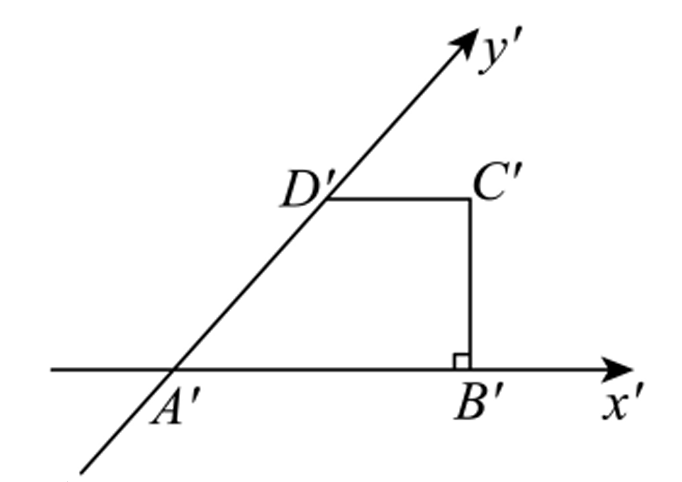
\includegraphics[width=0.3\linewidth]{figure/4.png}
}

% 5.
\begin{question}
  已知向量 $\vec{e}_1$, $\vec{e}_2$ 非零, 则 “$|\vec{e}_1+\vec{e}_2|=|\vec{e}_1|+|\vec{e}_2|$” 是 “存在非零实数 $m$, $n$, 使得 $m\vec{e}_1+n\vec{e}_2=0$” 的 \paren[A]
  \begin{choices}
    \item 充分不必要条件.
    \item 必要不充分条件.
    \item 充要条件.
    \item 既不充分也不必要条件.
  \end{choices}
\end{question}

% 6.
\begin{question}
  $D$ 是 $\mathrm{Rt}\triangle ABC$ 斜边 $BC$ 上一点, 若 $AB=AD$, $AC=\sqrt{3}DC$, 则 $\sin\angle ABC = $ \paren[D]
  \begin{choices}
    \item $\dfrac{1}{2}$
    \item $\dfrac{\sqrt{3}}{3}$
    \item $\dfrac{\sqrt{2}}{2}$
    \item $\dfrac{\sqrt{3}}{2}$
  \end{choices}
\end{question}

% 7.
\textfigure[fig-pos=right, text-width = 0.7\linewidth]{
  \begin{question}
    如图所示, 在边长为$4$的正八边形$ABCDEFGH$中, 点$O$是正八边形的中心, 点$P$是其内部任意一点. 则$\overrightarrow{OA}\cdot\overrightarrow{PA} + \overrightarrow{OF}\cdot\overrightarrow{PA}$的取值范围是 \paren[A]
    \begin{choices}
      \item $(-8\sqrt{2}, 16+8\sqrt{2})$.
      \item $(-16, 16+8\sqrt{2})$.
      \item $(-8, 16)$.
      \item $(-16, 16)$.
    \end{choices}
  \end{question}
  }{
  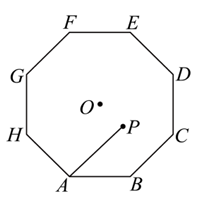
\includegraphics[width=0.3\linewidth]{figure/7.png}
}

% 8.
\begin{question}
  已知平行六面体$ABCD-A_1B_1C_1D_1$的所有棱长均为$2$, $O$为$AC$的中点, 且$A_1O\perp$平面$ABCD$, 若直线$AA_1$与底面$ABCD$的夹角为$45^\circ$, 则三棱锥$A-A_1BD$的外接球被平面$BCC_1B$截得的截面面积为 \paren[C]
  \begin{choices}
    \item $\frac{2\pi}{3}$.
    \item $\pi$.
    \item $\frac{4\pi}{3}$.
    \item $2\pi$.
  \end{choices}
\end{question}

\section{%
  多选题：本题共 3 小题，每小题 5 分，共 15 分。
  在每小题给出的选项中，有多项符合题目要求。
  全部选对的得 5 分，部分选对的得 2 分，有选错的得 0 分。
}

% 9.
\textfigure[fig-pos=right, text-width = 0.7\linewidth]{
  \begin{question}
    如图, 在平行四边形 $ABCD$ 中, $E$ 为 $CD$ 的中点, $\overrightarrow{AF}=\dfrac{1}{3}\overrightarrow{AE}$, 则 \paren[BCD]
    \begin{choices}
      \item $\overrightarrow{AE}=\overrightarrow{BC}-\dfrac{1}{3}\overrightarrow{BA}$.
      \item $\overrightarrow{BE}=\overrightarrow{BC}+\dfrac{1}{2}\overrightarrow{BA}$.
      \item $\overrightarrow{BF}=\dfrac{1}{3}\overrightarrow{BC}+\dfrac{5}{6}\overrightarrow{BA}$.
      \item $\overrightarrow{AE}+\overrightarrow{BE}=2\overrightarrow{BC}$.
    \end{choices}
  \end{question}
}{
  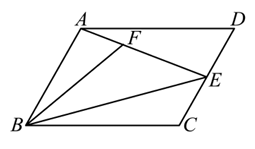
\includegraphics[width=0.3\linewidth]{figure/9.png}
}

% 10.
\begin{question}
  已知 $\triangle ABC$ 三个内角 $A,B,C$ 对边分别是 $a,b,c$, 若 $(\sqrt{3}c - 2a\sin B)\sin C = \sqrt{3}(b\sin B-a\sin A)$, 则下列选项正确的是 \paren[BCD]
  \begin{choices}
    \item $B=\dfrac{\pi}{6}$.
    \item 若 $D$ 是 $AC$ 边上的一点, 且 $\overrightarrow{CD}=2\overrightarrow{DA}$, $BD=2$, 则 $\triangle ABC$ 的面积的最大值为 $\dfrac{3\sqrt{3}}{2}$.
    \item 若 $\triangle ABC$ 是锐角三角形, 则 $\dfrac{c}{a}$ 的取值范围是 $\left(\dfrac{1}{2},2\right)$.
    \item 若 $O$ 是 $\triangle ABC$ 的外心, $\overrightarrow{OB}=m\overrightarrow{OA}+n\overrightarrow{OC}$, 则 $m+n\in[-2,1)$.
  \end{choices}
\end{question}

% 11.
\textfigure[fig-pos=right, text-width = 0.7\linewidth]{
  \begin{question}
    如图, 在矩形$ABCD$中, $AD=2AB=4$, $E$为$BC$的中点. 将$\triangle BAE$沿$AE$向上翻折到$\triangle PAE$, 连接$PC, PD$, 在翻折过程中, 下列说法正确的是 \paren[AD]
    \begin{choices}
      \item 若平面$PAE\perp$平面$ABCD$, 则$PA\perp DE$.
      \item 四棱锥$P-AECD$的体积最大值为$4\sqrt{2}$.
      \item 点$P$从点$B$翻折到$AD$中点的过程中, $PD$的中点$F$形成的轨迹长度为$\sqrt{2}\pi$.
      \item 三棱锥$P-AED$的外接球表面积的最小值为$16\pi$.
    \end{choices}
  \end{question}
}{
  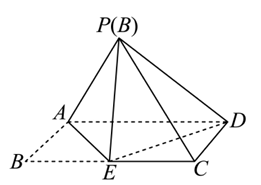
\includegraphics[width=0.3\linewidth]{figure/11.png}
}